

\begin{frame}{Do czego potrzebna jest mapa}
	Istnieje implementacja zadania nawigacji bez wykorzystania mapy, w tym wypadku jest to tak zwana nawigacja zliczeniowa. 
	Jej wykorzystanie powoduje jednak generowanie błędu pozycji, którego nie da się zniwelować,	a który rośnie z czasem.
	W celu minimalizacji tego rodzaju błędów wykorzystuje się cechy charakterystyczne środowiska \cite{robotics_vision_dead_reckon}, a więc mapę.
	To podejście do nawigacji jest wykorzystywane w opisywanej pracy inżynierskiej.
\end{frame}

\begin{frame}{Jak działa algorytm budowy mapy}
	\begin{itemize}
		\item początkowe założenie - znana pierwotna pozycja robota
		\item uzyskanie punktów otoczenia względem robota
		\item możliwość wykorzystania wielu czujników - systemu LiDAR, kamery Kinect, sonarów etc.
		\item możliwa identyfikacja poszczególnych punktów na mapie w celu późniejszego szybkiego ich rozpoznania lub przechowywanie jedynie współrzędnych zajętych obszarów
	\end{itemize}
\end{frame}

\begin{frame}{Na co pozwalają implementacje budowy mapy}
	\begin{columns}
		\begin{column}{0.5\textwidth}
			\begin{figure}
				\centering
				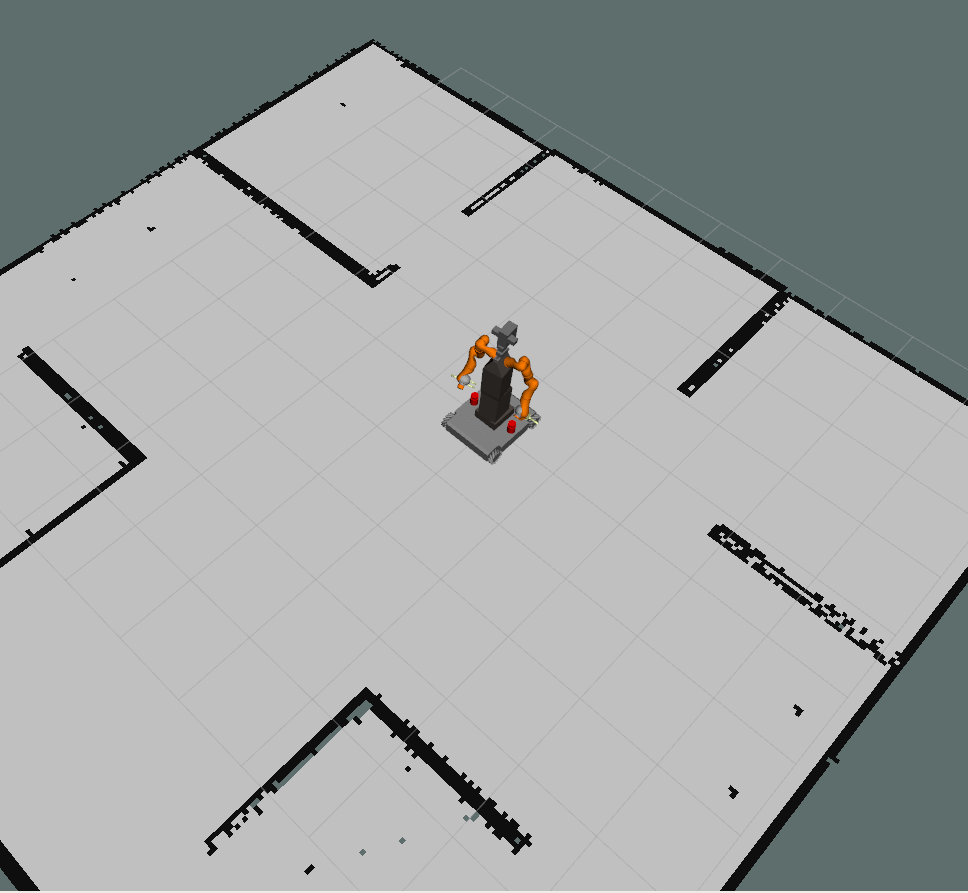
\includegraphics[height=0.6\textheight]{img/mapa_2d.png}
				\caption{dwuwymiarowa mapa zbudowana przy pomocy czujników LiDAR}
			\end{figure}
		\end{column}
		\begin{column}{0.5\textwidth}  %%<--- here
			\begin{figure}
				\centering
				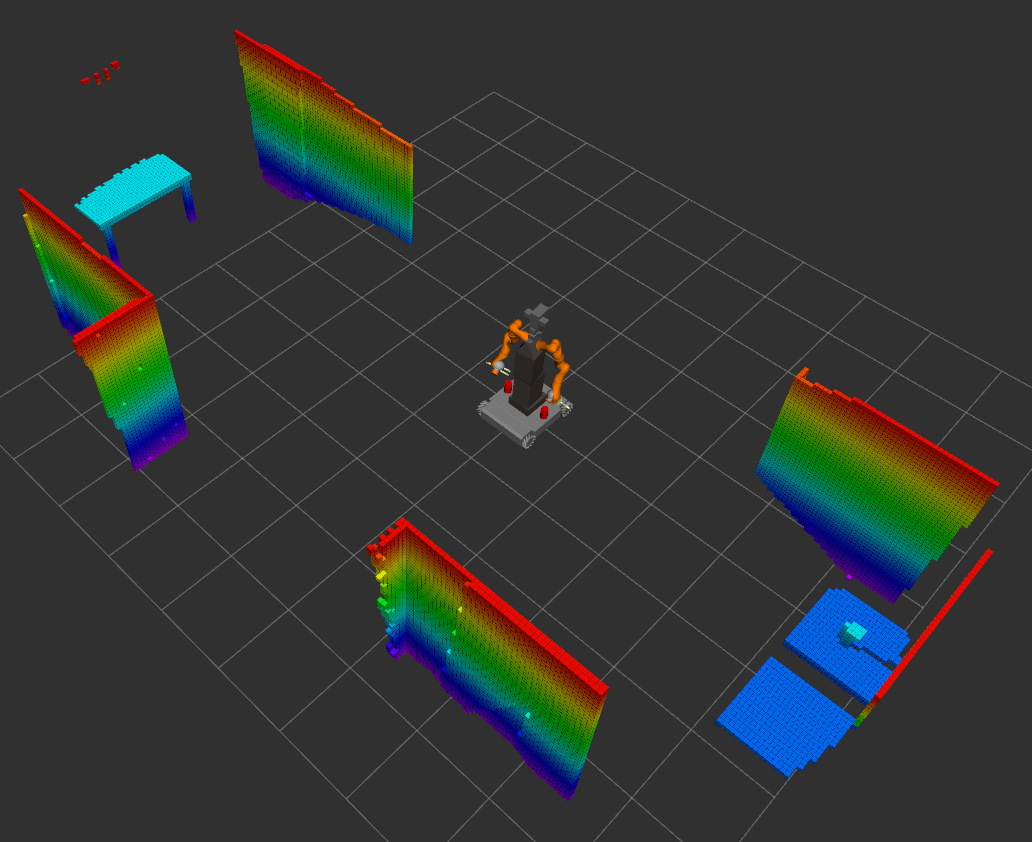
\includegraphics[height=0.6\textheight]{img/octomapa.png}
				\caption{mapa trójwymiarowa zbudowana za pomocą kamery Kinect}
			\end{figure}
		\end{column}
	\end{columns}
\end{frame}

\begin{frame}{Własności niektórych implementacji}
	\begin{columns}
		\begin{column}{0.5\textwidth}
			\begin{center}
				czujnik LiDAR
			\end{center}
			\begin{itemize}
				\item szybkie tworzenie obrazów dużych płaskich przestrzeni
				\item dane pobrane tylko na jednej wysokości, zwykle blisko podłoża (mapa 2D)
			\end{itemize}
		\end{column}
		\begin{column}{0.5\textwidth}  %%<--- here
			\begin{center}
				kamera Kinect
			\end{center}
			\begin{itemize}
				\item mniejszy kąt widzenia czujnika i wymagane większe zasoby - potrzeba więcej czasu, pamięci i cykli procesora do budowy takiej mapy				
				\item budowa obrazu trójwymiarowej przestrzeni
			\end{itemize}
		\end{column}
	\end{columns}
\end{frame}
